% DO NOT COMPILE THIS FILE DIRECTLY!
% This is included by the the driver file (FlipBeamerTemplate.tex).


{%% This is a total kludge for a fancy title page background
%\vspace{1.5em}

%% Opening.png is the Data61 black background
\setbeamertemplate{sidebar right}{\llap{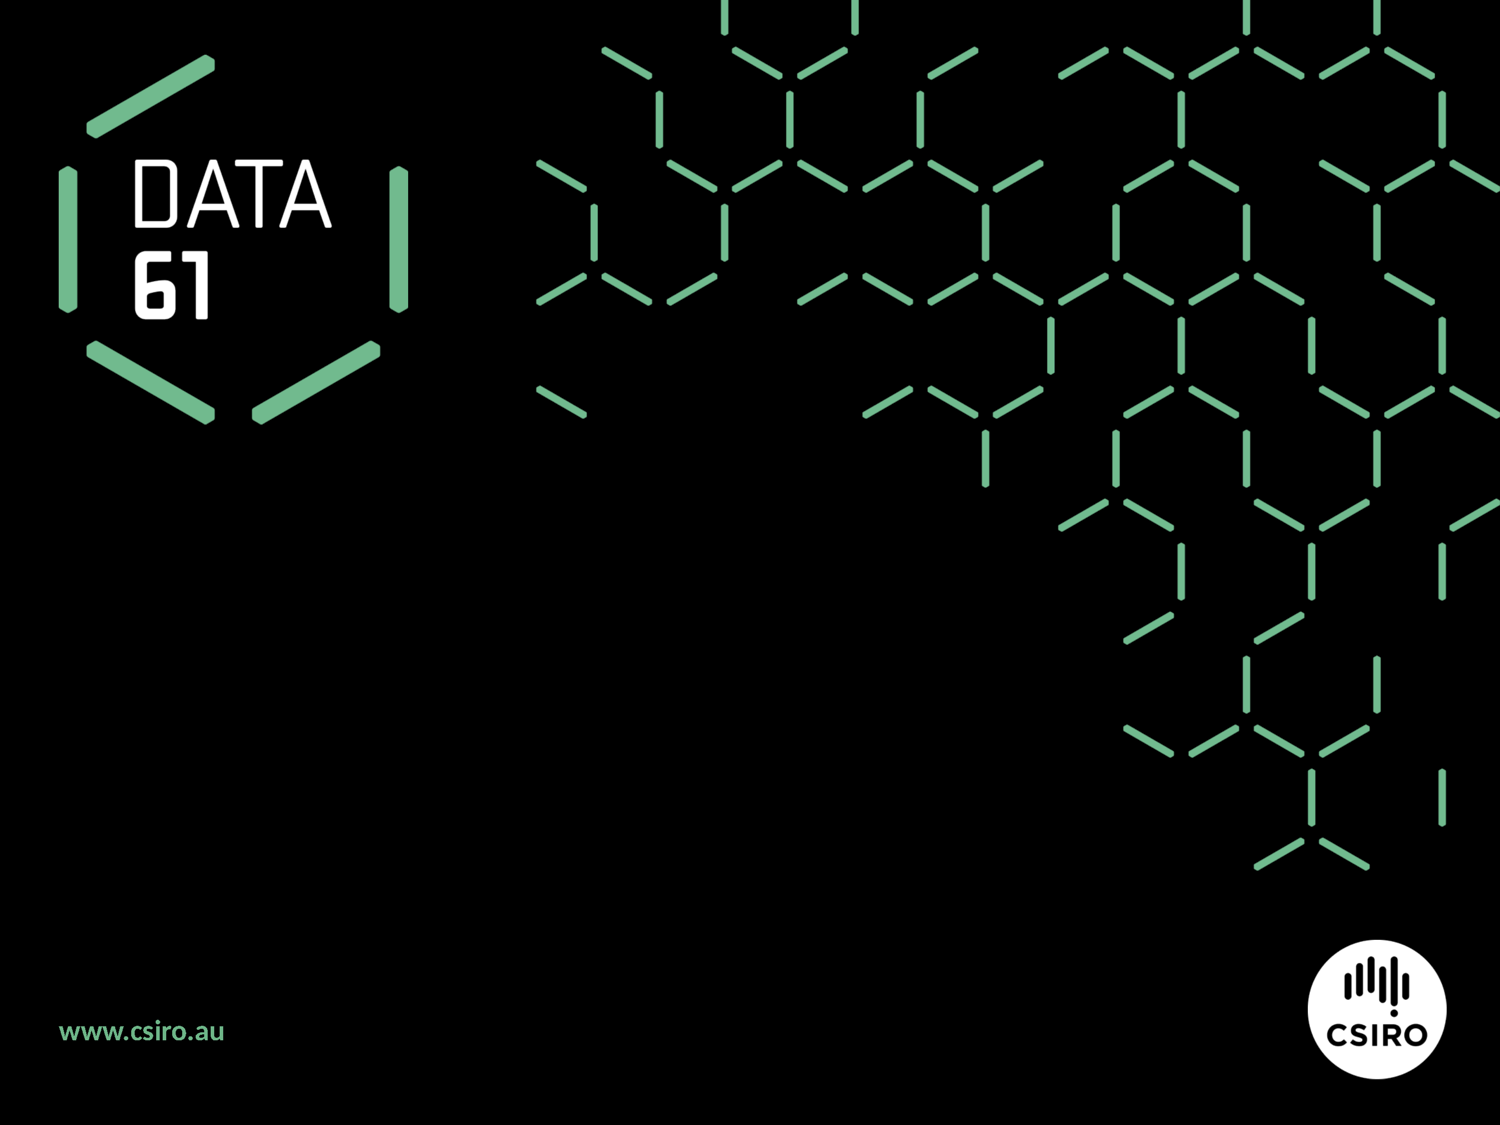
\includegraphics[width=\paperwidth,height=\paperheight]{Opening}}}
\begin{frame}[c]%{\phantom{title page}} 

\begin{center}
	
	\vspace{10em}
	\footnotesize\textcolor{gray}{Beamer Template: 	\texttt{Felipe Maldonado}}
	\vspace{.5em}
	
	%% Include the University logo
	
\includegraphics[height=1.5cm]{logoANU2011}\\
	\textcolor{anugold}{\textit{Australian National University}, \today} %% use the ANU gold color 

\end{center}
\end{frame}
}

%%%  Separator.png is the Data61 green background

%{
%\setbeamertemplate{sidebar right}{\llap{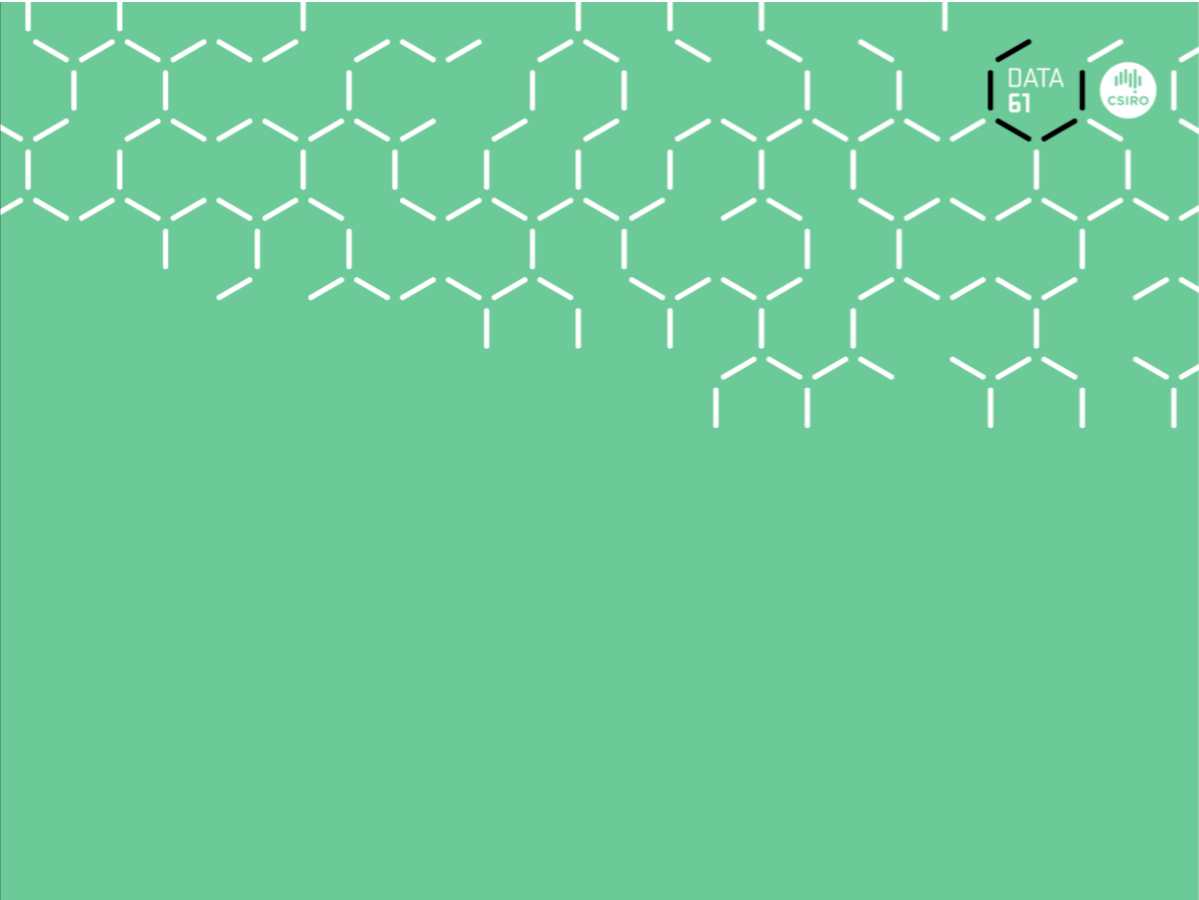
\includegraphics[width=\paperwidth,height=\paperheight]{separator}}}
\begin{frame}[c]{ \textit{Beamer template Data61/ANU:}}
\begin{itemize}
\item Contains two .tex files, one where you can include your content, and the other to compile (and define whatever package you need )
\item MUST compile using XeLaTeX
\item Already defined 3 colours: {\it anugold}: \textcolor{anugold}{anugold};   {\it dataplum}: \textcolor{dataplum}{data61 green};  {\it datagreen}: \textcolor{datagreen}{data61 darker green} 
\item By default the footbar is datagreen, the topbar (and the title) is anugold, and every slide has a background image containing both logos (+ a network). 
\item Support .png and .pdf images. 
\end{itemize}
\end{frame}
%}

 %%%%% Blocks %%%%%
\begin{frame}[c]{Blocks}{Different kinds of blocks}
	\begin{block}{Block}
		Normal block. Colorless, neutral.
	\end{block}

	\begin{exampleblock}{Example Block}
		Example block. (Potential uses: list of pros, relaxing facts)
	\end{exampleblock}

	\begin{alertblock}{Alert Block}
		Alert block. (Potential uses: list of cons, impending doom)
	\end{alertblock}
\end{frame}
	
	%%%%%%%SEPARATION%%%%%
	
	
\addtocounter{framenumber}{-1} %% Using this code we don?t increase the number of pages. And the counter skip this type of pages 
{	
\setbeamertemplate{sidebar right}{\llap{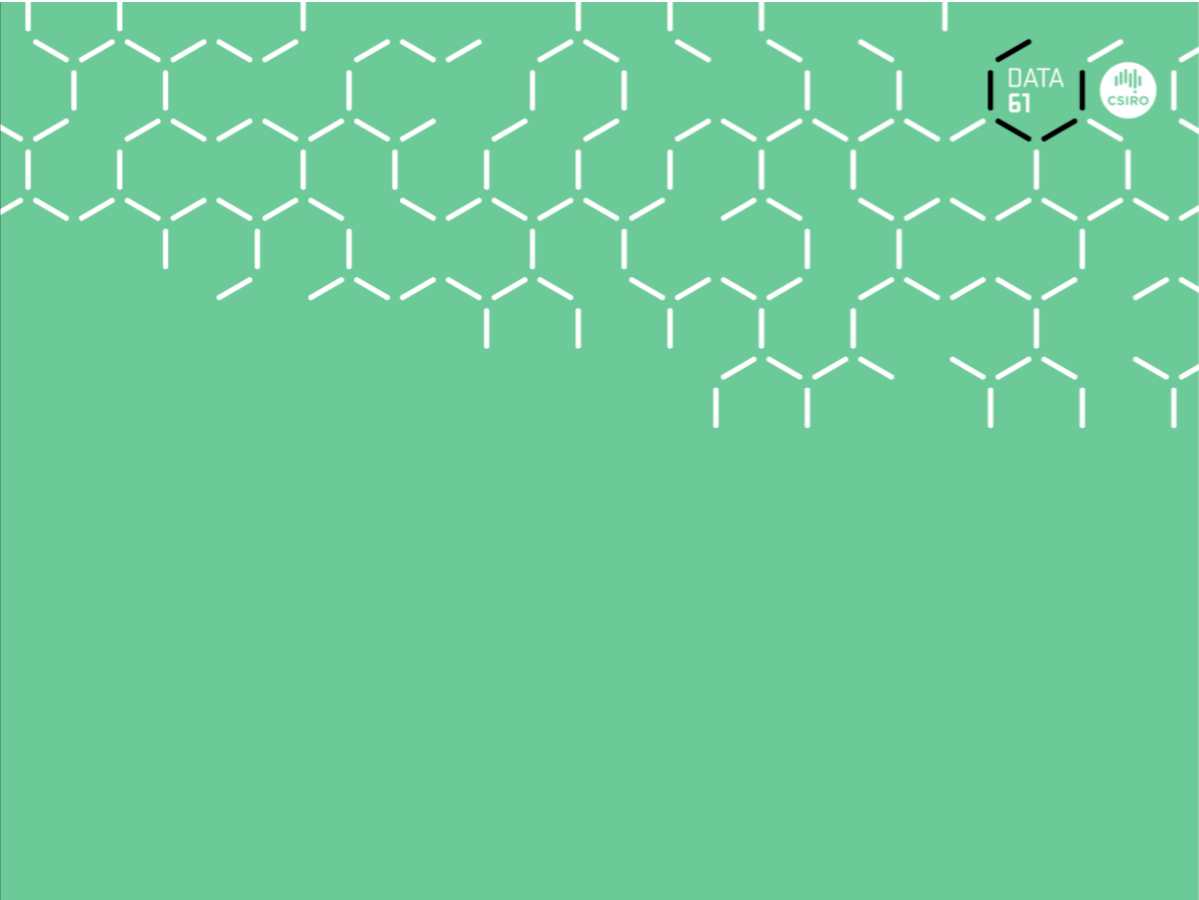
\includegraphics[width=\paperwidth,height=\paperheight]{separator}}}  %% Separator.png is the Data61 green background
\begin{frame}[c]
\vspace{10em}
This is a transition slide, it does not increase the number of pages (see the content.tex file to learn how to use it).


\end{frame}
}
	
	

%%%%%%%MODEL AND ASSUMPTIONS 1 %%%%%%
\begin{frame}[c]{Title}{Subtitle}
More colours already defined:
		\begin{columns}[t]
		\begin{column}[T]{5.5cm}
			\begin{itemize}
			\item This is \textcolor{crimsonred}{crimsonred}.
			\item This is \textcolor{paleale}{paleale} / \textcolor{lager}{lager}.
			\item This is \textcolor{turtlegreen}{turtlegreen} / \textcolor{green}{green}.
			\item This is \textcolor{paleblue}{paleblue}.
			\end{itemize}
		\end{column}

		\begin{column}[T]{5.5cm}
			\begin{itemize}
			\item This is \textcolor{gray}{gray}.
			\item This is \textcolor{charcoal}{charcoal}.
			\item This is \textcolor{jeans}{jeans}.
			\item This is \textcolor{regal}{regal}.
			% \item This is \textcolor{keynotetop}{keynotetop}.
			\end{itemize}
		\end{column}
		\end{columns}
		\vspace{1em}

You can use the \alert{\texttt{textcolor}} command to use these, but the goal is to do things in a way where there are no calls to explicit colors, just user-adjustable values.
\end{frame}



%%%%%%%MODEL AND ASSUMPTIONS 2 %%%%%%
\begin{frame}[c]{Sample Feynman Diagrams}
	Using \texttt{tikzfeynman.sty}, you can draw Feynman diagrams with ease. \comment{The default color follows the normal text, so it automatically changes color when you swap from a light to a dark background.}
	
	\begin{center}
	\begin{tikzpicture}[line width=1.5 pt, scale=.6]
		\draw [fermionbar]		(-3,1.5) -- (-2,.75);
		\draw [fermionbar]		(-2,.75) -- (-1,0);
		\draw [fermionbar]		(-1,0) -- (-2,-.75);
		\draw [fermionbar]		(-2,-.75) -- (-3,-1.5);
		\draw [vector]			(-1,0) -- (1,0);
		\draw [fermionbar]		(2,-1.5) -- (1,0);
		\draw [fermionbar]		(1,0) -- (2,1.5);
		\draw [scalar, dash pattern=on 5pt off 4pt]			(-2,.75) -- (-2,-.75);
	\end{tikzpicture}
	\usebeamercolor[fg]{title}
	\begin{tikzpicture}[line width=1.5 pt, scale=.6]
		\draw [fermionbar]		(-3,1.5) -- (-2,.75);
		\draw [fermionbar]		(-2,.75) -- (-1,0);
		\draw [fermionbar]		(-1,0) -- (-2,-.75);
		\draw [fermionbar]		(-2,-.75) -- (-3,-1.5);
		\draw [vector]			(-1,0) -- (1,0);
		\draw [fermionbar]		(2,-1.5) -- (1,0);
		\draw [fermionbar]		(1,0) -- (2,1.5);
		\draw [scalar, dash pattern=on 5pt off 4pt]			(-2,.75) -- (-2,-.75);
	\end{tikzpicture}
	\usebeamercolor[fg]{normal text}
	\begin{tikzpicture}[line width=1.5 pt, scale=.6]
		\draw [fermionbar]		(-3,1.5) -- (-2,.75);
		\draw [fermionbar]		(-2,.75) -- (-1,0);
		\draw [fermionbar]		(-1,0) -- (-2,-.75);
		\draw [fermionbar]		(-2,-.75) -- (-3,-1.5);
		\draw [vector, color=ALERT]			(-1,0) -- (1,0);
		\draw [fermionbar]		(2,-1.5) -- (1,0);
		\draw [fermionbar, color=FMGreen]		(1,0) -- (2,1.5);
		\draw [scalar, dash pattern=on 5pt off 4pt]			(-2,.75) -- (-2,-.75);
	\end{tikzpicture}
	\end{center}
	\vspace{1em}
	This makes it easy to copy and paste TikZ code from your paper! You can also import diagrams as images. Be sure to use an empty background and pdf/png format to ensure transparency.  
	
	
	\usebeamercolor[fg]{normal text} 
	% Don't forget to include this when you're done futzing with colors
\end{frame}


\begin{frame}[c]{Other diagrams}
	Here's a nice picture illustrating Seiberg duality:
	\vspace{.5em}
	\begin{center}
		\begin{tikzpicture}[line width =1.5, scale=.8]
			\draw[fill] (0,0) circle (.075);
			\draw[fermion] (0,0) -- (2.5,0);
			\draw[fermionbar] (2.5,0) -- (4.5,0);
			\draw[dashed] (4.5,0) -- (5.5,0) node[right] {$g$};
			\draw[fill] (2.5,0) circle (.075);
			\node[below] at (2.5,0) {$g_*$};
			%
			\draw[fermion] (0,3) -- (0,0);
			\draw[dashed] (0,3) -- (0,3.5) node[above] {$y$};
			%
			% Bezier Curve!
			\draw[fermion, line width=1] (.3,3) .. controls (.7,.2) and (.75,.2) .. (3,2);
			\draw[fermion, line width=1, color=alert] (0,0) to [out=15, in=240] (3,2);
			\draw[fermion, line width=1, color=ALERT] (2.5,0) -- (3,2);
			\draw[fermion, line width=1] (4.5,.2) .. controls (3,.7) and (3.2,.4) .. (3,2);
			%
			\draw[fill] (3,2) circle (.075);
			\draw[fermion, line width=1] (.5,3) .. controls (1,1) and (1.2,1) .. (3,2);
			\draw[fermion, line width=1] (4.5,3) .. controls (3,2.5) and (3.5,2.5) .. (3,2);
			\draw[fermion, line width=1] (1.5,3) to [out = -20, in = 110] (3,2);
			\node[right] at (3,2) {\textcolor{COMMENT!75!white}{$(\hat g, \hat y)$}};
		\end{tikzpicture}	
	\end{center}
	\vspace{.5em}
	Image based on Strassler's `unorthodox' review of SUSY gauge theory.
\end{frame}



%%%%%%%%SEPARATOR%%%%%%%%% BACKGROUND
\addtocounter{framenumber}{-1}
{	
\setbeamertemplate{sidebar right}{\llap{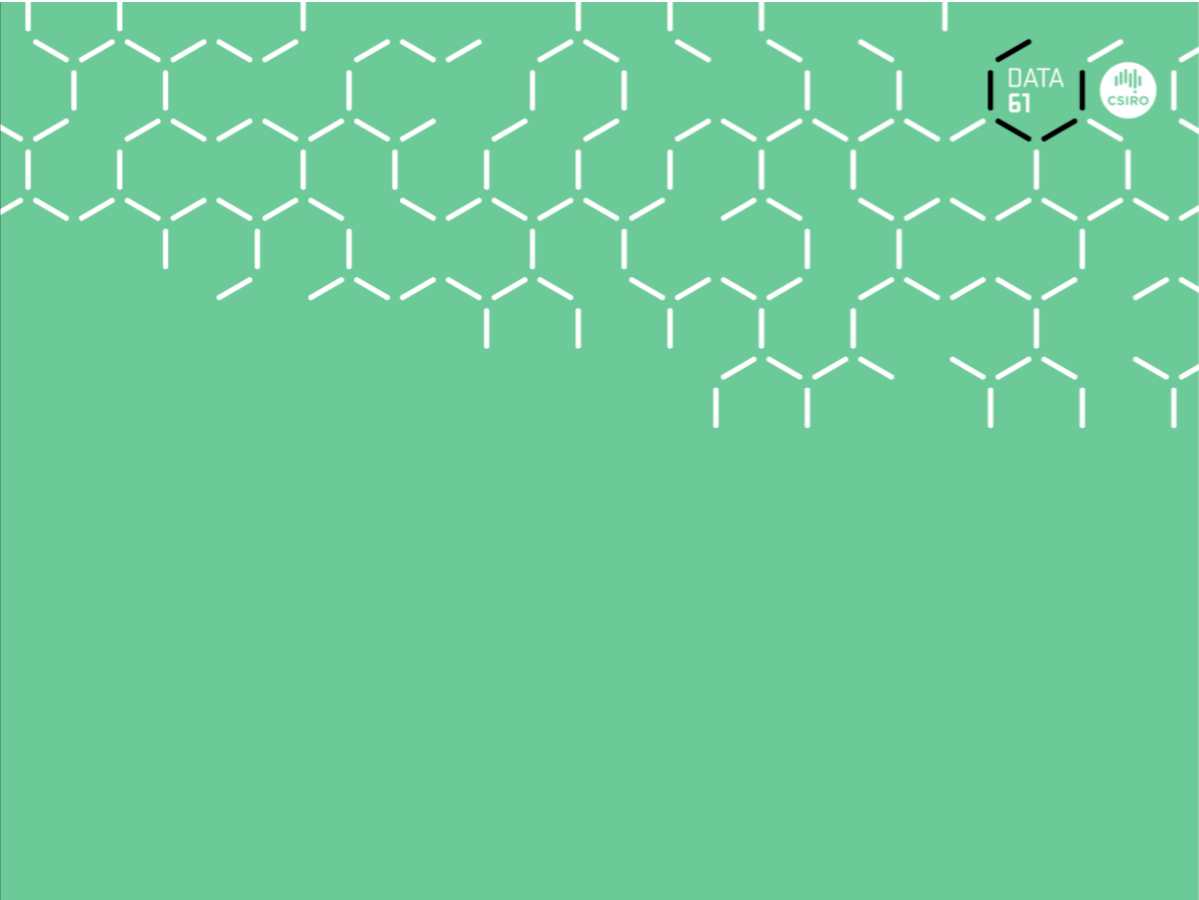
\includegraphics[width=\paperwidth,height=\paperheight]{separator}}}
\begin{frame}[c]
\vspace{9.5em}

You will need to adjust the text/images to some suitable position.
\begin{center}

	\vspace{.5em}
	 
\includegraphics[height=1.5cm]{Background}\\
	\vspace{.5em}
	
\end{center}
\end{frame}
}
	
%%%%%% Stochastic Approx.	
 
\begin{frame}[c]{Equations}{...and theorems}
\begin{block}{Definition: Robbins-Monro Algorithm}A {\it Robbins-Monro
    Algorithm} (RMA) is a discrete time stochastic processes
  $\{x_k\}_{k \geq 0}$ whose general structure is specified by
\begin{equation}
\label{RMA}
x_{k+1}-x_k=\gamma_{k+1}[F(x_k)+U_{k+1}],
\end{equation}
\noindent	
where
\begin{itemize}
\item $x_k$ takes its values in some Euclidean space (e.g., $\R^n$ );
\item $\gamma_k$ is deterministic and satisfies $\gamma_k>0$,
  $\sum_{k \geq 1}\gamma_k=\infty$, and $\lim_{k \to\infty}\gamma_k=0$;
\item $F:\R^n\to\R^n$ is a deterministic continuous vector field;
\item $\EE[U_{k+1}| \Fk]=0$, where $\Fk$ is the natural filtration of
  the entire process.%\footnote{Because of this last condition on
%    $U^k$, a Robbins-Monro Algorithm is also known as a {\it
%      Martingale Difference Stochastic Approximation}.}
\end{itemize}
\end{block}
	
\end{frame}	
	
	
	
%%%%%%%% THE ODE METHOD






%%%%%%%%%%dynamic equilibria %%%%%

\begin{frame}[c]{Equilibria}
\begin{exampleblock}{Theorem 2.} 
\label{eqs}
Let $f(x)=x^r, 0<r<1$. Then, there is a unique equilibrium to Equation \eqref{RMC-MS} 
in $int(\Delta^{n-1})$, the interior of the simplex, specified by 
\[
\phi^*=\dfrac{1}{\sum_j
  \overline{q}_j^{\frac{1}{1-r}}}[\overline{q}_1^{\frac{1}{1-r}},...,\overline{q}_n^{\frac{1}{1-r}}]
\]
The remaining equilibria are on the boundary of the simplex.
\end{exampleblock}


\textcolor{anugold}{\textit{Remark:}}
If assume that there exists a set $Q\subset \{1,..,n\}$
($|Q|<n$) of indexes such that $\phi_i=0$ if $i\in Q$. The remaining coordinates are given as follows: If $j \notin
Q$, then we have
\[
\phi_j=\frac{\overline{q}_j^{1/(1-r)}}{\sum_{i\notin Q}\overline{q}_i^{1/(1-r)}}.
\]

%
%\begin{exampleblock}{Lemma 2.}
%\label{induction}
%Consider a trial-offer market defined by $n$ items and the submarket
%obtained by considering only $n-1$ items.  This submarket can also be
%modeled by an RMA. 
%\end{exampleblock}
\end{frame}


%%%%%%%%%%CONVERGENCE r<1, UNSTABILITY r>1%%%%%

\begin{frame}[c]{Equilibria and stability}
\begin{exampleblock}{Main Theorem} 
\label{thm:ict} 
Under the social signal $f(x)=x^r, 0<r<1$ with $\phi^0\in
int(\Delta^n)$, the RMA $\{\phi^t\}_{t>0}$ converges to $\phi^*$
almost surely.
\end{exampleblock}

\begin{center}
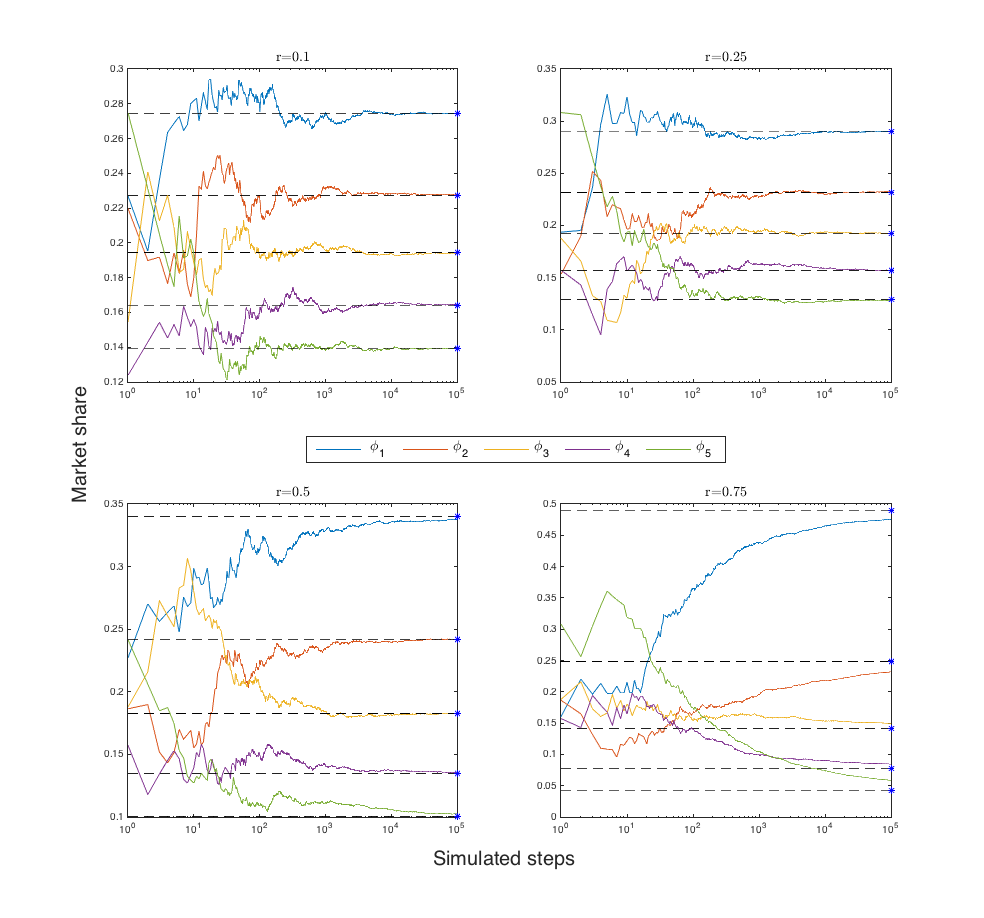
\includegraphics[scale=0.2]{Convergence10x5ItIND}
\end{center}



\end{frame}


%%%%%%%%%%PLOTS PREDICT%%%%%

\begin{frame}[c]{Plots}
\begin{center}
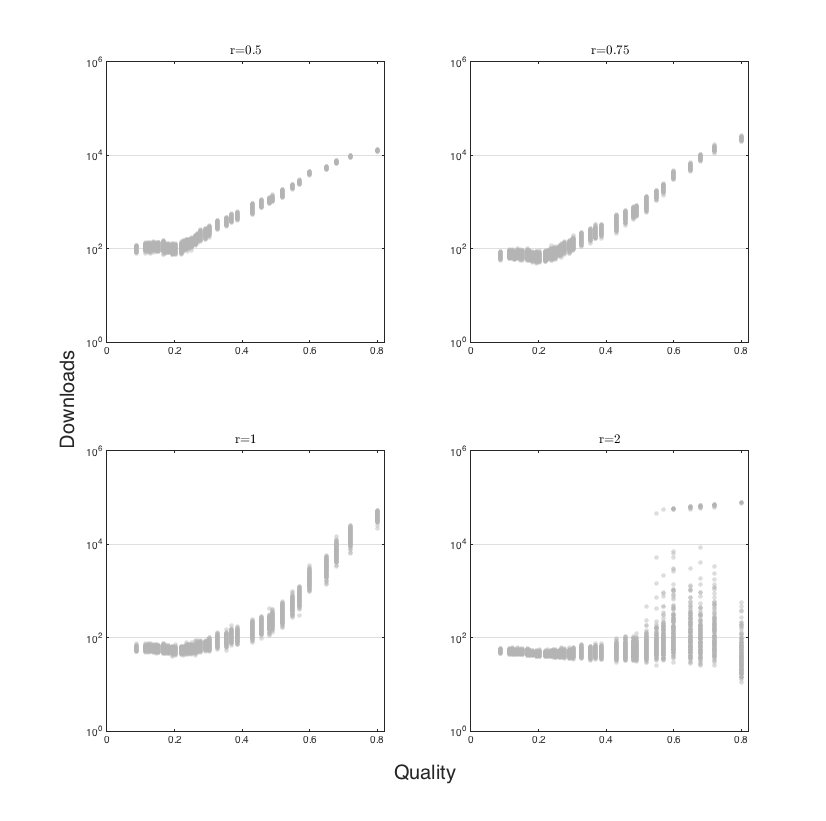
\includegraphics[scale=0.3]{predict200expeNegCorrQrank10x5it}
\end{center}


\end{frame}



{	
\setbeamertemplate{sidebar right}{\llap{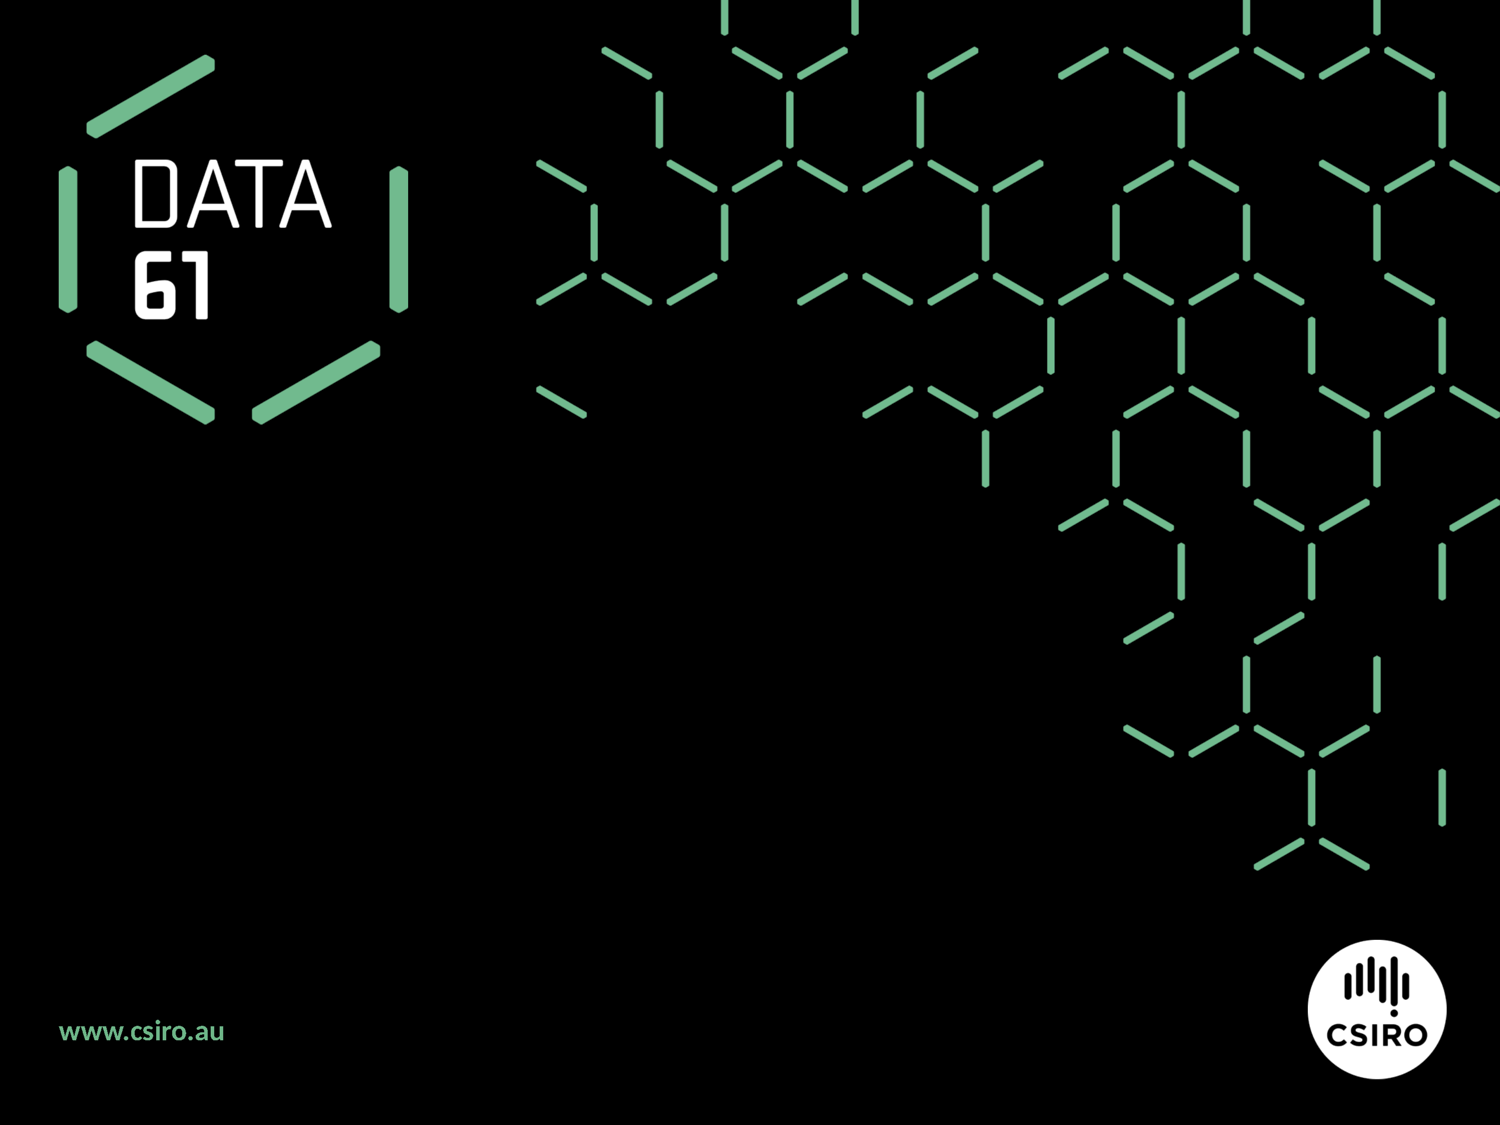
\includegraphics[width=\paperwidth,height=\paperheight]{Opening}}}
\begin{frame}[c]{Last slide}
\begin{center}

	\vspace{10em}
	 
\includegraphics[height=1cm]{Thanks}\\
	\vspace{.5em}
	
\end{center}
\end{frame}
}


%%%BACKUP SLIDES 1

\addtocounter{framenumber}{-1}
{
\begin{frame}[c]{Backup slides} 
{\it Proof of Theorem 2}
We know the equilibria are given by $p(x)=x\Leftrightarrow p_i(x)=x_i, \forall i\in\{1,...,K\} $, then
	
%%%% equilibria	
	$p_i(\Phi)=\phi_i\Leftrightarrow \frac{\overline{q}_i(\phi_i)^r}{\sum_{j=0}^K\overline{q}_j(\phi_j)^r}=\phi_i$\\
	if  $\phi_i>0$ for all $i$, and then we have the following:
	$p_i(\Phi)=\phi_i\Leftrightarrow \overline{q}_i(\phi_i)^{r-1}=\sum_{j=0}^K\overline{q}_j(\phi_j)^r,$\\
	then 	\begin{equation*}
	\overline{q}_i(\phi_i)^{r-1}=\overline{q}_j(\phi_j)^{r-1}\Leftrightarrow \phi_i=\left(\frac{\overline{q}_i}{\overline{q}_j}\right)^{\frac{1}{1-r}}\phi_j
	\end{equation*}
	
	Adding from $i=1$ to $i=K$ we have
	$1=\sum_{i=1}^K\phi_i=\frac{\phi_j}{\overline{q}_j^{1/(1-r)}}\sum_{i=1}^K\overline{q}_i^{1/(1-r)},$
	and in consecuence
	$\phi_j=\frac{\overline{q}_j^{1/(1-r)}}{\sum_{i=1}^K\overline{q}_i^{1/(1-r)}},\quad j\in \{1,...,K\} $ are the coordinates of the equilibrium.

\end{frame}



%%%BACKUP SLIDES 2

\addtocounter{framenumber}{-1}
{
\begin{frame}[c]
{\it Proof of Theorem 3}
The proof studies the asymptotic behaviour of the solutions of the following ODE:
\begin{equation}
\label{ODEE}
\frac{d \phi^t}{dt}=p(\phi^t)-\phi^t.
\end{equation}

Hence, we have
\begin{align*}
&\frac{\overline{q}_i(\phi_i^t)^r}{\sum_j\overline{q}_j(\phi_j^t)^r}=\frac{d\phi_i^t}{d t}+\phi_i^t, \\
&\frac{1}{\sum_j\overline{q}_j(\phi_j^t)^r}=\frac{1}{\overline{q}_i(\phi_i^t)^r}[\frac{d\phi_i^t}{d t}+\phi_i^t] \quad \mbox{ if } \phi_i^t\neq 0,\\
&\overline{q}_i^{-1}[(\phi_i^t)^{-r}\frac{d\phi_i^t}{d t}+(\phi_i^t)^{1-r}]=\overline{q}_j^{-1}[(\phi_j^t)^{-r}\frac{d\phi_j^t}{d t}+(\phi_j^t)^{1-r}], \\
&\frac{d}{dt}\left[ e^{(1-r)t}\overline{q}_i^{-1}(\phi_i^t)^{1-r}\right]=\frac{d}{dt}\left[ e^{(1-r)t}\overline{q}_j^{-1}(\phi_j^t)^{1-r}\right]
\end{align*} 



\end{frame}
}



%%%BACKUP SLIDES 3

}\addtocounter{framenumber}{-1}
{
\begin{frame}[c]
Integrating and re-ordering  terms we have:
\begin{equation}
\label{equili}
\frac{(\phi_i^t)^{1-r}}{\overline{q}_i}-\frac{(\phi_j^t)^{1-r}}{\overline{q}_j}= e^{(r-1)t}\left[   \frac{(\phi_i^0)^{1-r}}{\overline{q}_i}-\frac{(\phi_j^0)^{1-r}}{\overline{q}_j} \right].
\end{equation}

if $\displaystyle
  \frac{(\phi_i^0)^{1-r}}{\overline{q}_i}\neq\frac{(\phi_j^0)^{1-r}}{\overline{q}_j}$,
  the right-hand side of Equation \eqref{equili} goes to zero as $t\to \infty$  (because
  $r<1$) and hence
\begin{equation}
\label{limit}
\lim_{t\to\infty} \frac{(\phi_i^t)^{1-r}}{\overline{q}_i}-\frac{(\phi_j^t)^{1-r}}{\overline{q}_j}=0. 
\end{equation}

Now denote by $\phi_j$ the limit of $\phi_j^t$ for all $j \in
\{1,...,n\}$. Using Equation \eqref{limit}, the following equation holds for all $i,j
\in\{1,...,n\}$:
\begin{equation}
\frac{\phi_{i}^{1-r}}{\overline{q}_i}=\frac{\phi_{j}^{1-r}}{\overline{q}_j} \Leftrightarrow \phi_{i}=\frac{\phi_{j}}{\overline{q}_j^{1/(1-r)}}\overline{q}_i^{1/(1-r)}
\end{equation}

which is the equation that defines $\phi^*$ in Theorem 2.

\end{frame}
}

